% This file was created with tikzplotlib v0.10.1.
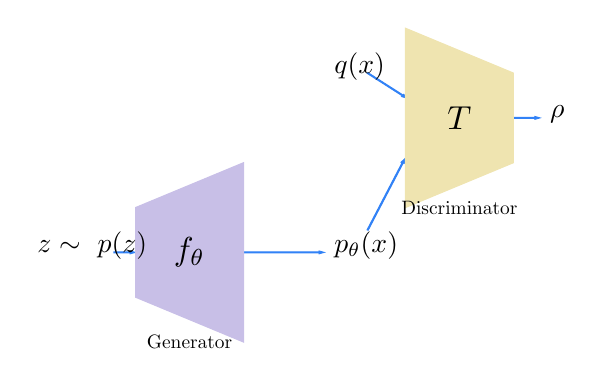
\begin{tikzpicture}

\definecolor{darkgray176}{RGB}{176,176,176}
\definecolor{dodgerblue50130246}{RGB}{50,130,246}
\definecolor{palegoldenrod239228176}{RGB}{239,228,176}
\definecolor{thistle200191231}{RGB}{200,191,231}

\begin{axis}[
hide x axis,
hide y axis,
tick align=outside,
tick pos=left,
x grid style={darkgray176},
xmin=0, xmax=10,
xtick style={color=black},
y grid style={darkgray176},
ymin=0, ymax=10,
ytick style={color=black}
]
\path [draw=dodgerblue50130246, fill=dodgerblue50130246]
(axis cs:1.99,4)
--(axis cs:1.9,3.97)
--(axis cs:1.9,3.99)
--(axis cs:1.6,3.99)
--(axis cs:1.6,4.01)
--(axis cs:1.9,4.01)
--(axis cs:1.9,4.03)
--cycle;
\path [draw=dodgerblue50130246, fill=dodgerblue50130246]
(axis cs:5.49,4)
--(axis cs:5.4,3.97)
--(axis cs:5.4,3.99)
--(axis cs:4,3.99)
--(axis cs:4,4.01)
--(axis cs:5.4,4.01)
--(axis cs:5.4,4.03)
--cycle;
\path [draw=dodgerblue50130246, fill=dodgerblue50130246]
(axis cs:6.98578466938709,6.08258000627789)
--(axis cs:6.9775266687593,5.98807177687097)
--(axis cs:6.9591755562531,5.99602392562366)
--(axis cs:6.3091755562531,4.49602392562366)
--(axis cs:6.2908244437469,4.50397607437634)
--(axis cs:6.9408244437469,6.00397607437634)
--(axis cs:6.9224733312407,6.01192822312903)
--cycle;
\path [draw=dodgerblue50130246, fill=dodgerblue50130246]
(axis cs:7.02133615901941,7.44512603152353)
--(axis cs:6.93170867717451,7.47622128032686)
--(axis cs:6.9439028923915,7.49207376010895)
--(axis cs:6.2939028923915,7.99207376010895)
--(axis cs:6.3060971076085,8.00792623989105)
--(axis cs:6.9560971076085,7.50792623989105)
--(axis cs:6.96829132282549,7.52377871967314)
--cycle;
\path [draw=dodgerblue50130246, fill=dodgerblue50130246]
(axis cs:9.49,7)
--(axis cs:9.4,6.97)
--(axis cs:9.4,6.99)
--(axis cs:9,6.99)
--(axis cs:9,7.01)
--(axis cs:9.4,7.01)
--(axis cs:9.4,7.03)
--cycle;
\path [draw=thistle200191231, fill=thistle200191231]
(axis cs:4,2)
--(axis cs:4,6)
--(axis cs:2,5)
--(axis cs:2,3)
--cycle;
\path [draw=palegoldenrod239228176, fill=palegoldenrod239228176]
(axis cs:7,9)
--(axis cs:7,5)
--(axis cs:9,6)
--(axis cs:9,8)
--cycle;
\draw (axis cs:3,2) node[
  scale=0.7,
  text=black,
  rotate=0.0
]{Generator};
\draw (axis cs:8,5) node[
  scale=0.7,
  text=black,
  rotate=0.0
]{Discriminator};
\draw (axis cs:0,4) node[
  anchor=base west,
  text=black,
  rotate=0.0
]{$z\sim~p(z)$};
\draw (axis cs:5.5,4) node[
  anchor=base west,
  text=black,
  rotate=0.0
]{$p_\theta(x)$};
\draw (axis cs:5.5,8) node[
  anchor=base west,
  text=black,
  rotate=0.0
]{$q(x)$};
\draw (axis cs:9.5,7) node[
  anchor=base west,
  text=black,
  rotate=0.0
]{$\rho$};
\draw (axis cs:3,4) node[
  scale=1.2,
  text=black,
  rotate=0.0
]{$f_\theta$};
\draw (axis cs:8,7) node[
  scale=1.2,
  text=black,
  rotate=0.0
]{$T$};
\end{axis}

\end{tikzpicture}
